%energieEffizienz.tex

\section*{Gliederung}
\begin{frame}{Gliederung}
\tableofcontents
\end{frame}

\section{Stand der globalen Energietransformation}
\label{s.stand}
	\begin{frame}
	\frametitle{Stand: Net Zero Roadmap}
	\framesubtitle{\hspace*{\fill}iea (International Energy Agency)\cite{iea_net_zero2023}}
	
	\begin{itemize}
	 \item saubere Energietechnologien 
		  \begin{itemize}
			  \item verändern die Aussichten für Emissionen 
		    \item durch politische Maßnahmen, expandierende Märkte und sinkende Kosten
				\item selbst unter den derzeitigen politischen Rahmenbedingungen
		\end{itemize}
		\pause
		\item Verringerung der  Emissionen  voraussichtlich um \textbf{7,5 Gt } in 2030    
			 \begin{itemize}
		   	 \item bezogen auf das  Basisszenario vor Paris aus dem Jahr 2015
			   \item Szenario STEPS (Stated Policies Scenario)  
				 \item 5 Gt  Ausbau der Photovoltaik und der Windkraft und 
				 \item fast 1 Gt durch  Elektrofahrzeuge 
			 \end{itemize}
			\pause
			\item  die prognostizierte Erwärmung von 2,4 $^\circ$C im Jahr 2100 \textbf<2->{besorgniserregend} hoch 
			\begin{itemize}
				\item unter den derzeitigen politischen Rahmenbedingungen 
				\item \textbf<2->{aber} um 1 $^\circ$C niedriger liegt als vor dem Pariser Abkommen im Jahr 2015.
     \end{itemize}
	\end{itemize}
		
	\end{frame}	
		
		
\begin{frame}{Stand: Net Zero Roadmap}
	\framesubtitle{Globale \COz-Emissionen des Energiesektors \hspace*{\fill}
	                 iea (International Energy Agency)\cite{iea_net_zero2023}}
	
	
	\centering
	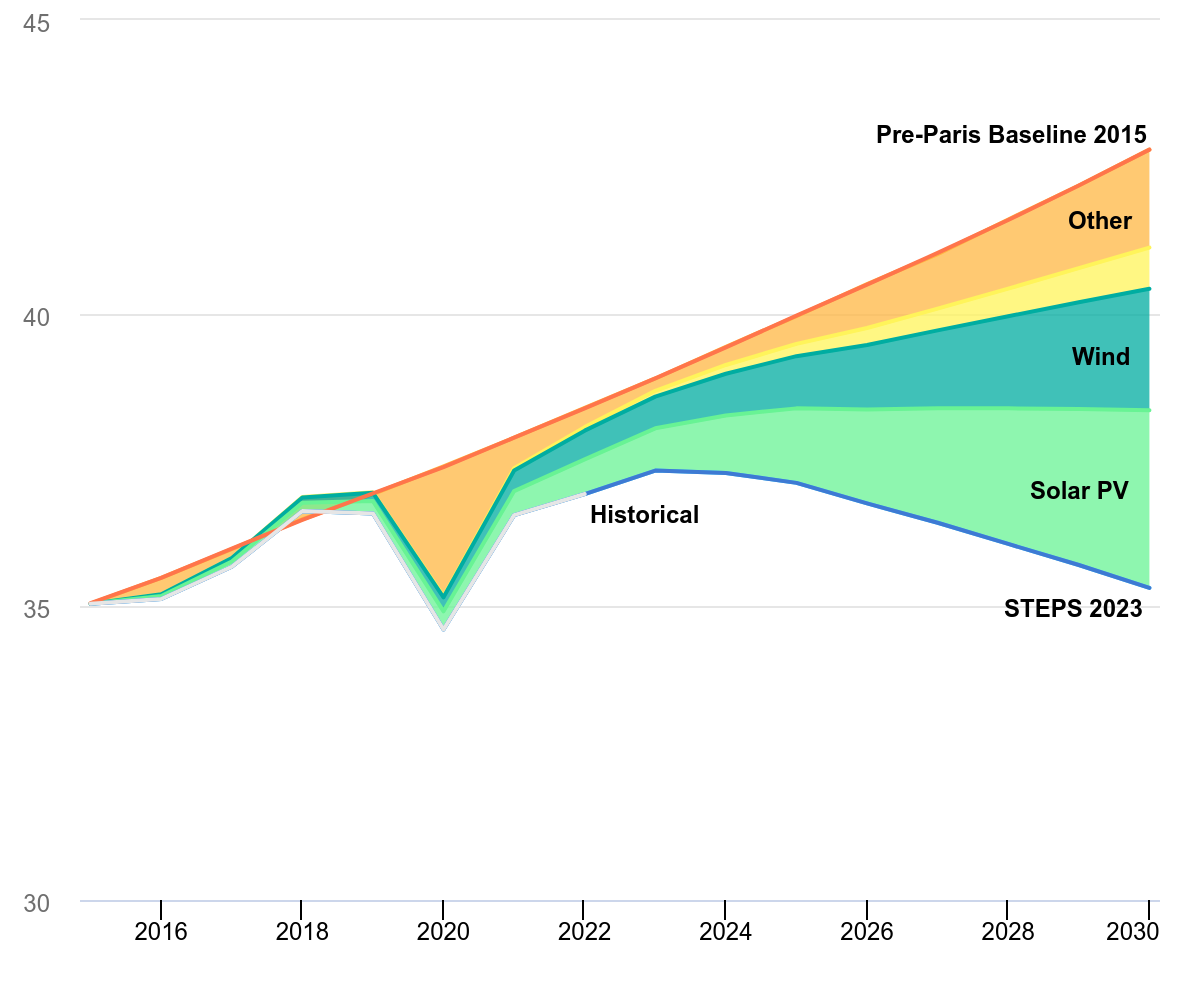
\includegraphics[width=.5\textwidth]{global-energy-sector-co2-emissions-in-the-pre-paris-baseline-and-stated-policies-scenarios-2015-2030.png}\label{fig.iea_co_em}\infoAbb
			%IEA (2023), Global energy sector CO2 emissions in the Pre-Paris Baseline and Stated Policies Scenarios, 2015-2030, IEA, Paris https://www.iea.org/data-and-statistics/charts/global-energy-sector-co2-emissions-in-the-pre-paris-baseline-and-stated-policies-scenarios-2015-2030, Licence: CC BY 4.0
	\end{frame}	
		
		
\begin{frame}{AR6 Synthesis Report: Climate Change 2023}
\framesubtitle{\hspace*{\fill} \href{https://www.ipcc.ch/report/sixth-assessment-report-cycle/}{\tiny https://www.ipcc.ch/report/sixth-assessment-report-cycle/} \cite{AR6_2024}}


		\centering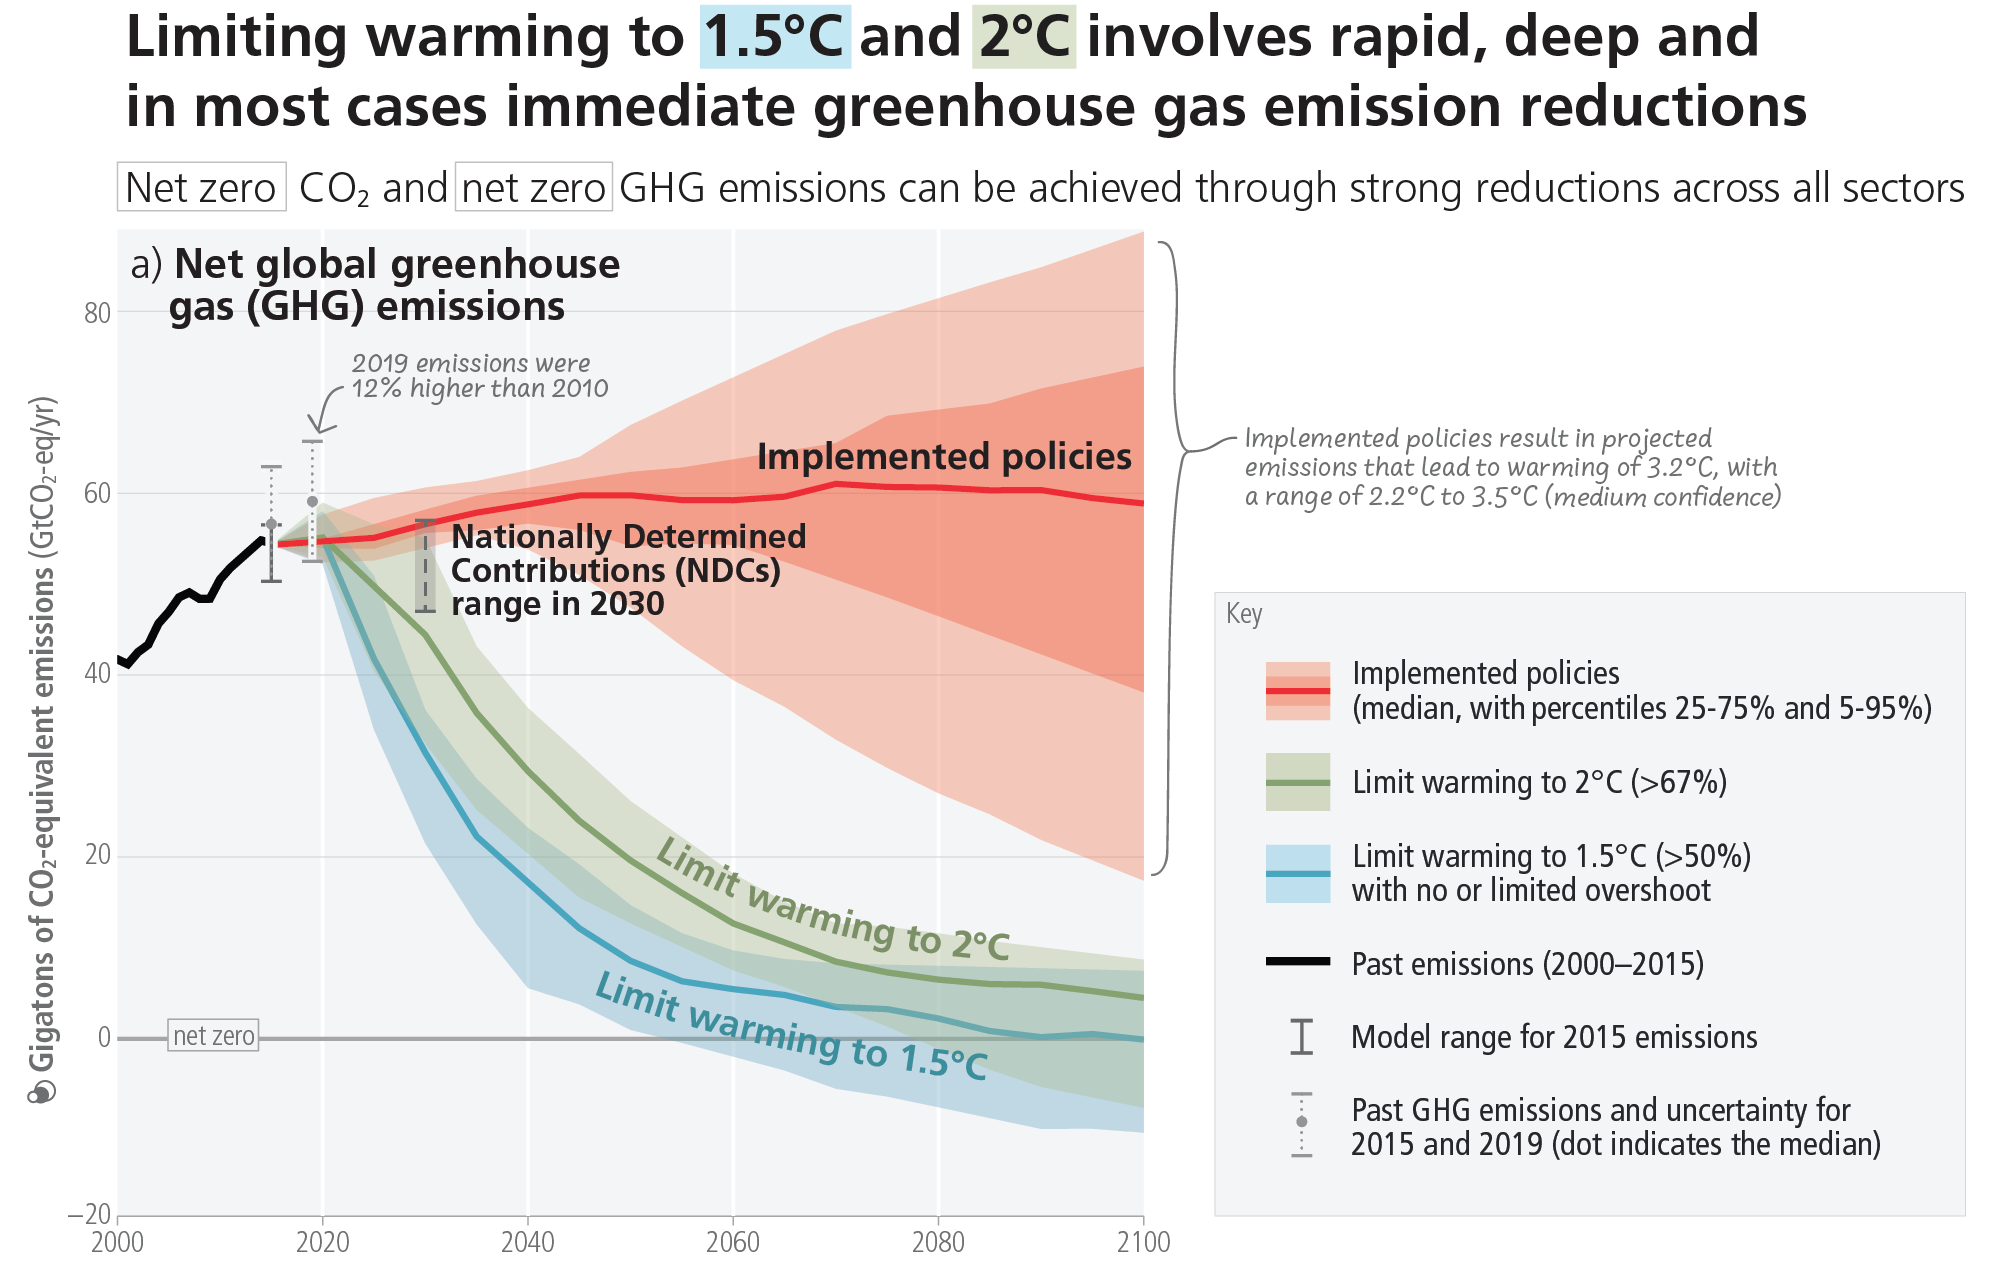
\includegraphics[width=.7\textwidth]{IPCC_AR6_SYR_SPM_Figure5.png}
		\label{fig.AR6_IPCC} \infoAbb
%Data supplied for archiving by the Technical Support Unit (TSU) for the Intergovernmental Panel on Climate Change (IPCC) Synthesis Report (SYR). Data curated on behalf of the IPCC Data Distribution Centre (IPCC-DDC).
%https://report.ipcc.ch/ar6syr/pdf/IPCC_AR6_SYR_SPM.pdf
%CC BY 4.0 Deed
%Attribution 4.0 International 

\end{frame}


\section{\COz \ und  IT}
\label{s.CO2_IT}

\begin{frame}{Gliederung}
\tableofcontents[currentsection]
\end{frame}

\begin{frame}{Auswirkungen digitaler Technologien}
%
\textbf{Digitale Technologien verursachen 2\% \\\hspace*{\fill}
                      der energiebezogenen Treibhausgasemissionen (THG)}
		\begin{itemize}
				\item direkte Auswirkungen auf Energieverbrauch und Emissionen
					\begin{itemize}
						\item rund 330 Mt \COze \ in 2020 
						\item durch Rechenzentren, Datenübertragungsnetze und vernetzten Geräte 
						\item 0,9\% der energiebezogenen THG-Emissionen  
				 \end{itemize}
			\pause
			\item geringe Steigerung der Emissionen seit 2010
				\begin{itemize}
					\item trotz der schnell wachsenden Nachfrage   
					\item Verbesserungen der Energieeffizienz, 
					\item Kauf von erneuerbaren Energien durch IKT-Unternehmen 
					\item umfassendere Dekarbonisierung der Stromnetze 
				\end{itemize}
				\pause 
			\item Aber \textbf<4->{Halbierung der Emissionen bis 2030}  für  Netto-Null-Emissionen bis 2050 (NZE) Szenario 
		\end{itemize}
		
\uncover<1->{\href{https://www.iea.org/energy-system/decarbonisation-enablers/digitalisation\#tracking}{\tiny https://www.iea.org/energy-system/decarbonisation-enablers/digitalisation\#tracking}}

\end{frame}

\begin{frame}{Energieverbrauch IT in Deutschland  \cite{grunwald_energy_2022} S.2}
	\begin{center}
	     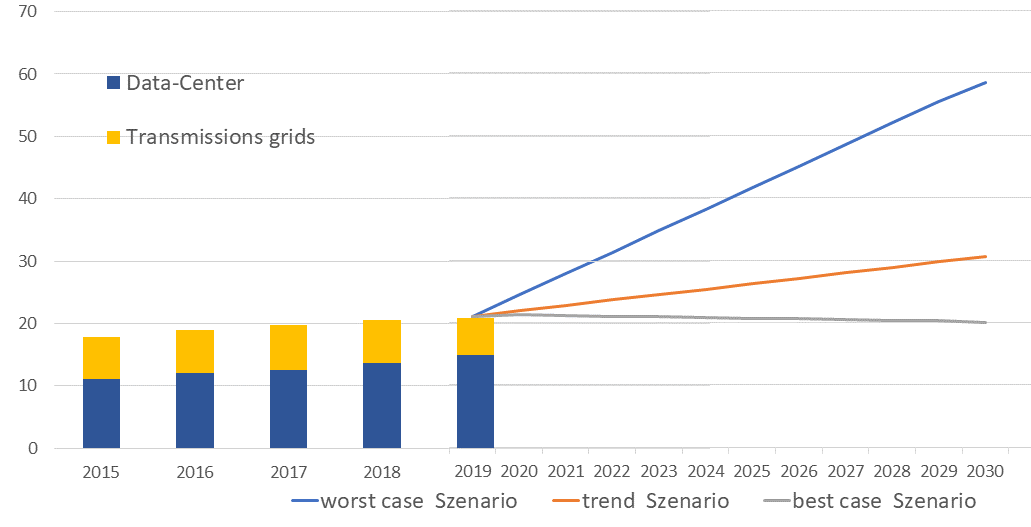
\includegraphics[width=.8\textwidth]{fignachTAB22.png}\label{fig.fignachTAB22}\infoAbb
			%nach [GC22] S.2
%Energy consumption of {ICT} infrastructure https://publikationen.bibliothek.kit.edu/1000152733
%Grünwald, Reinhard and Caviezel, Claudio
%2022
%doi: 10.5445/IR/1000152733
%ISSN: 2364-2645
	\end{center}

\end{frame}

\section{Digitaler \COz-Fußabdruck im Alltag}
\label{s.digFuss}

\begin{frame}{Gliederung}
\tableofcontents[currentsection]
\end{frame}

\begin{frame}{Wie sieht mein digitaler \COz-Fußabdruck aus?}
     \framesubtitle{Jeder für sich selbst hier: 
		          \href{https://www.digitalcarbonfootprint.eu/}{https://www.digitalcarbonfootprint.eu/} }
	\centering
	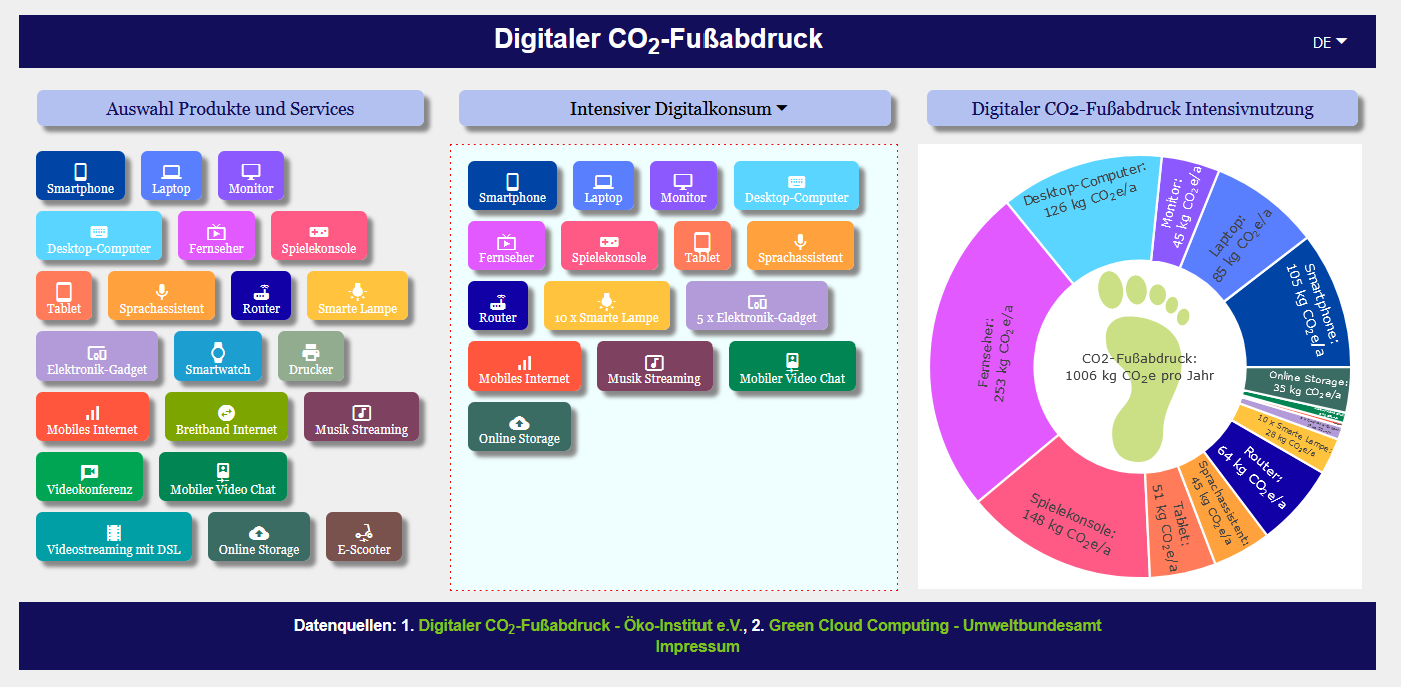
\includegraphics[width=.8\textwidth]{digit_CO2_FussAbruck.png}\label{fig.digit_CO2_FussAbruck}\infoAbb
\end{frame}


\begin{frame}{\COze-Emissionen  für Herstellung digitaler Endgeräte}
  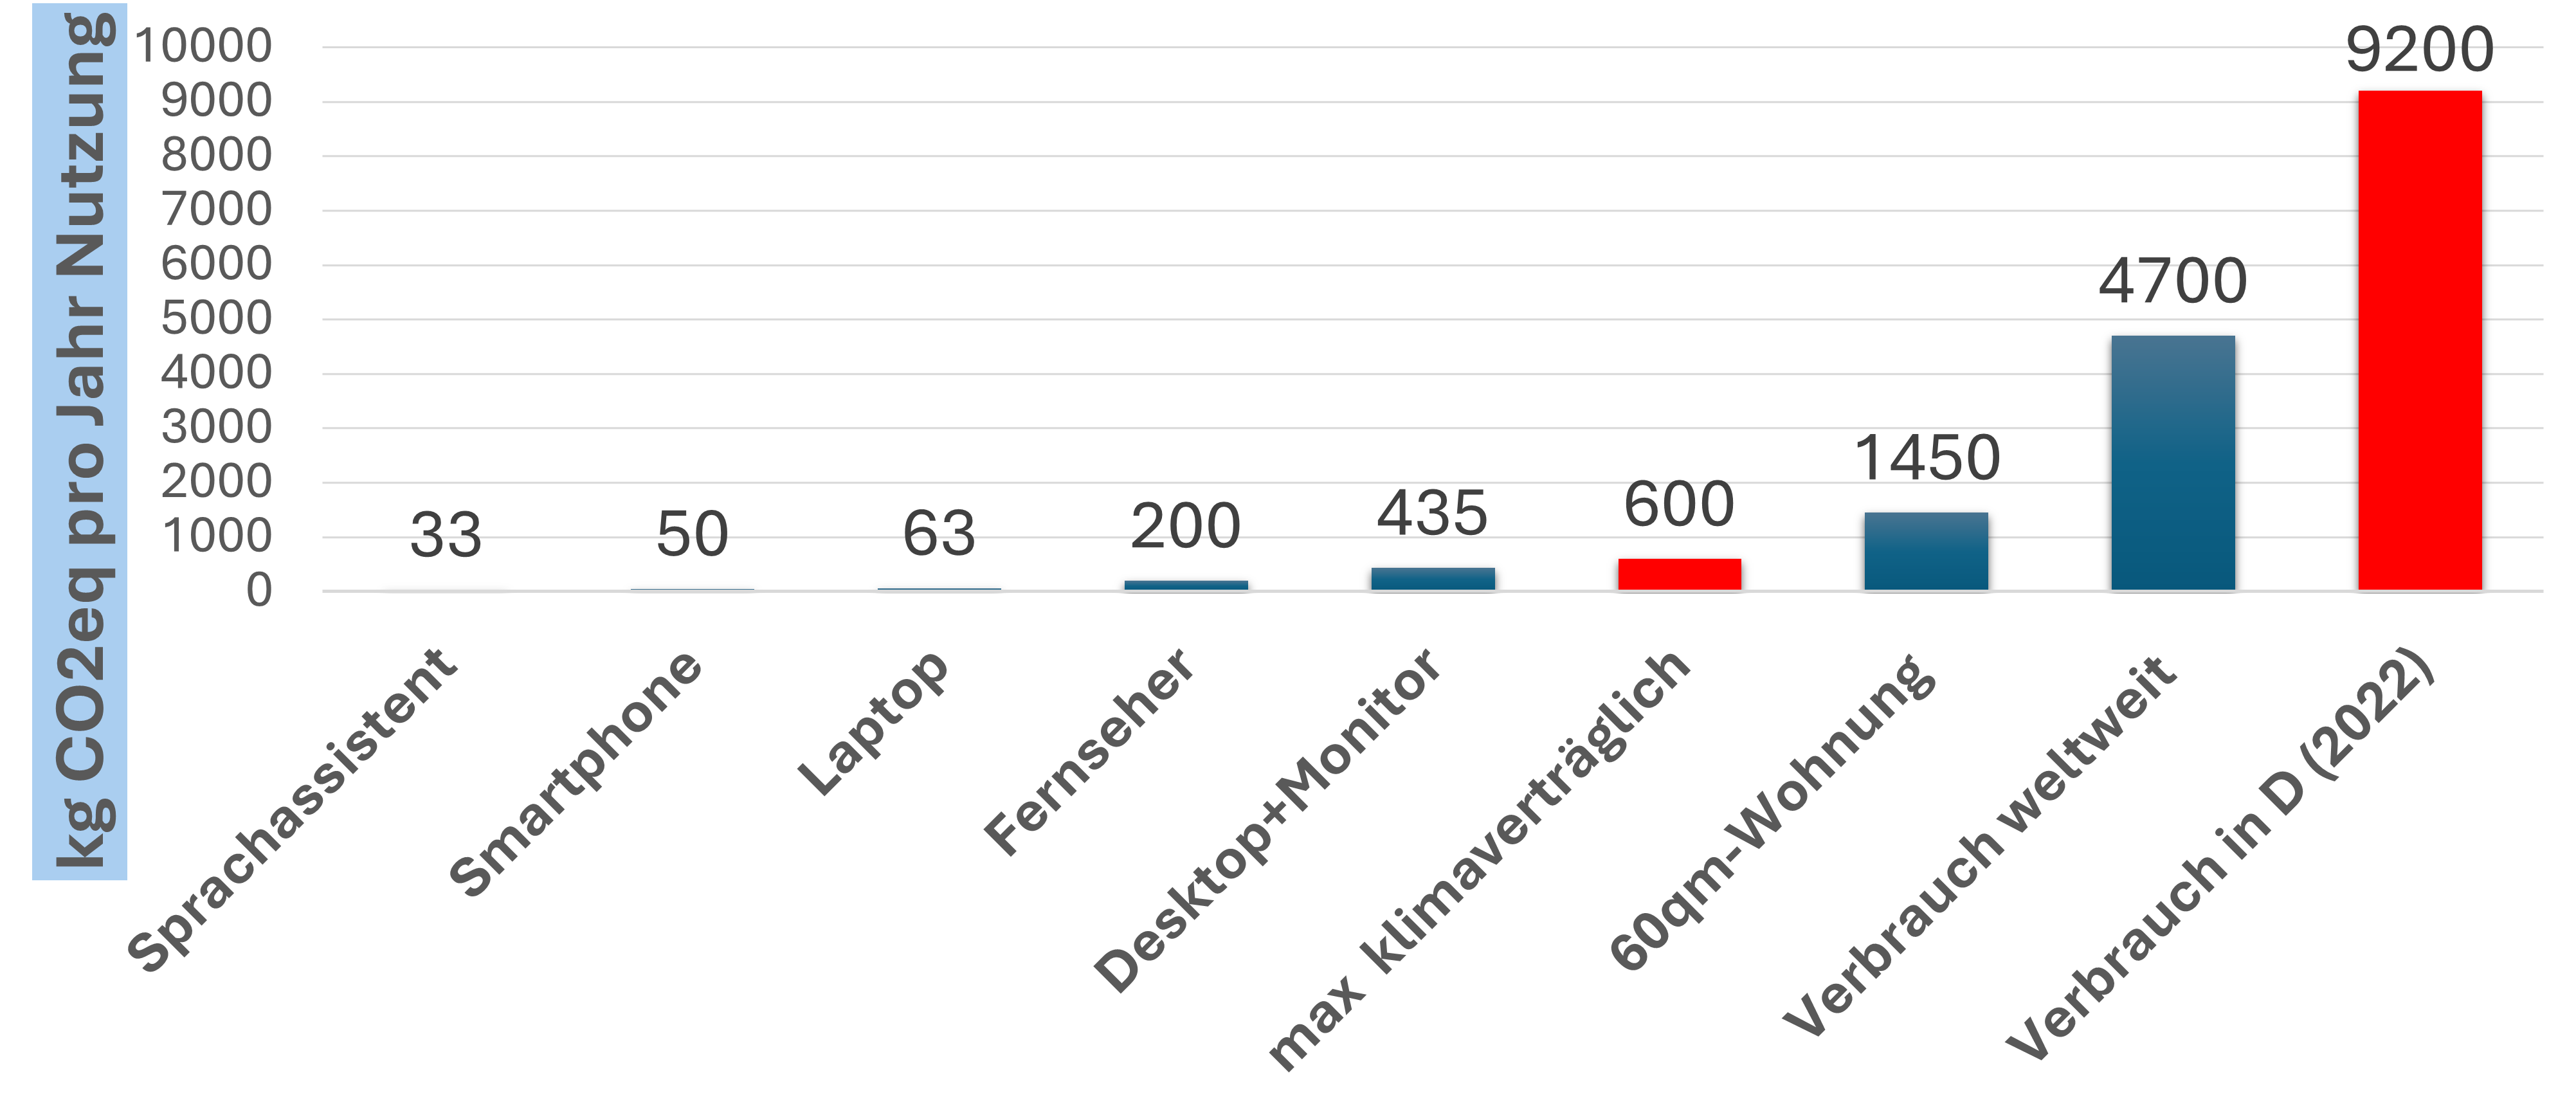
\includegraphics[width=.9\textwidth]{CO2_digEndg.png} \\ \hspace*{\fill}
	\label{fig.CO2_digEndg}\infoAbb
	% Daten siehe infoAbb und CO2eq_DigitalerAktionen.xlsx, erzeugt mit Adobe FireFly
\end{frame}
	
\begin{frame}{\COze-Emission für digitale Aktionen}		
		\centering
		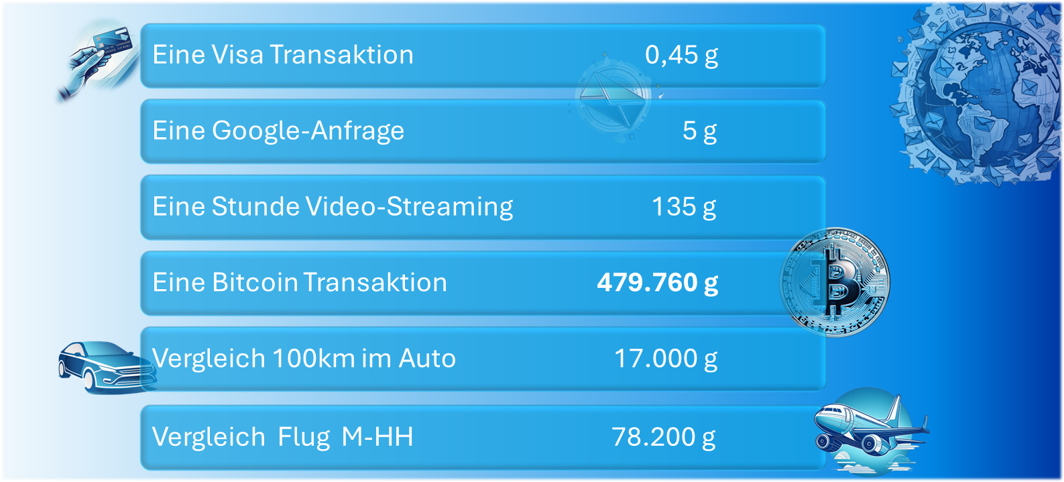
\includegraphics[width=.9\textwidth]{CO2_digiAktpng.png} \\ \hspace*{\fill}
	\label{fig.CO2_digiAkt}\infoAbb
		%		Eigene Illustration, Daten siehe infoAbb und CO2eq_DigitalerAktionen.xlsx, erzeugt mit Adobe FireFly
\end{frame}		



\section{(\COz-)effiziente Software}
\label{s.CO2_SW}

\begin{frame}{Gliederung}
\tableofcontents[currentsection]
\end{frame}

\begin{frame}{Was ist kohlendioxid- (\COz-) effiziente Software}
	\framesubtitle{\hspace*{\fill}oder grüne, nachhaltige, ressourcen-effiziente....SW}
	\begin{block}{}
	Im Softwarebereich besteht unsere Rolle bei der Lösung des Klimaproblems \textbf<2->{wenigstens} 
	in der Entwicklung kohlendioxid-effizienter Anwendungen. 
	
	Kohlendioxid-Effizienz bedeutet, Anwendungen zu entwickeln,\textbf<2->{ die uns oder unseren  
	Nutzern den gleichen Mehrwert bieten}, aber weniger Kohlendioxid \COz \ ausstoßen.
	\end{block}\pause 
	~\\[-10mm]\hspace*{\fill}
	\href{https://www.freepngimg.com/png/77530-emoticon-thinking-thought-world-whatsapp-day-emoji}{%	
	
\includegraphics[width=3cm]{emoji-thought.png}}\label{fig.emoji}
	%Lydia Simmons
	% Creative Commons (CC BY-NC 4.0) 
	%
\end{frame}

\begin{frame}{Digitale Suffizienz (\cite{santarius_digital_2023})} 
Grundlage dafür,  wie IKT zum  grundlegenden ökologischen Wandels beitragen kann 
\begin{itemize}[<+->]
	\item Hardwaresuffizienz: \\
	   weniger Geräte produzieren \\
		ihr absoluter Energiebedarf so gering wie möglich
  \item  Softwaresuffizienz:\\
	   Datenverkehr und die Hardwareauslastung während der Anwendung so gering wie möglich
 \item Nutzersuffizienz:\\
      digitale Geräte sparsam einsetzen \\
			IKT in einem nachhaltigen Lebensstil nutzen
\item Ökonomische Suffizienz:\\
    Digitalisierung für  Übergang zu einer Wirtschaft mit
		Wirtschaftswachstum nicht mehr als primäres Ziel, \
		ausreichende Produktion und ausreichenden Verbrauch innerhalb der planetarischen Grenzen
\end{itemize}

\end{frame}

\begin{frame}{\COz-effiziente Software}

\begin{itemize}
	\item ressourcenschonende und 
	\item \emph{energie-effiziente Softwareprodukte}
	\item auf älterer Hardware laufend und 
	\item  auf älterer Hardware  zu aktualisieren
	\item mit einem hohen Maß an Transparenz und Autonomie
\end{itemize}

\end{frame}


\begin{frame}{\COz-effiziente Software}
\framesubtitle{\hspace*{\fill}\href{https://learn.greensoftware.foundation/measurement}{https://learn.greensoftware.foundation/measurement}\cite{green_SW_pract_2024}}
		\begin{overprint}
			 \onslide<1>	  
				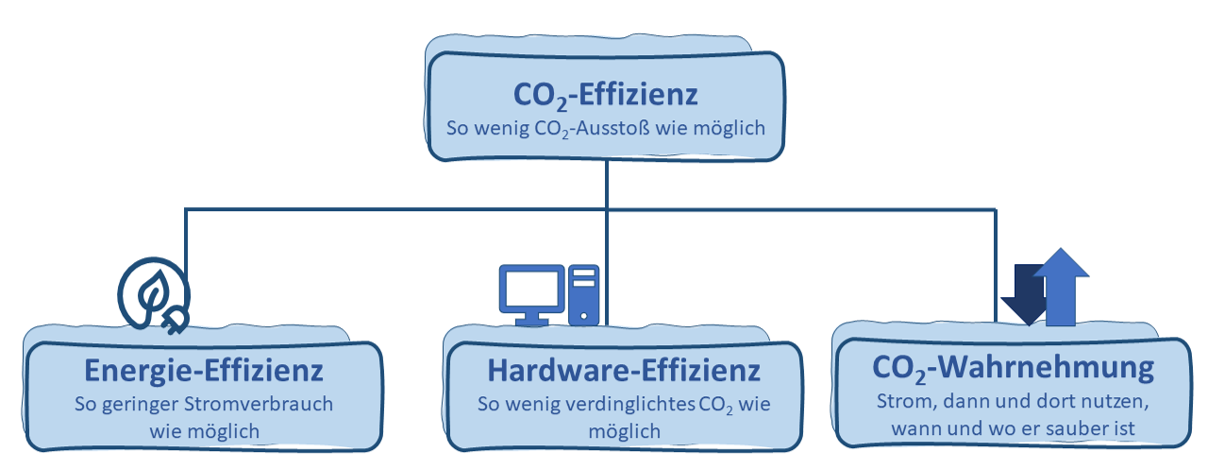
\includegraphics[width=1.00\textwidth]{CO2awa_1.png}
				%Autorin nach https://learn.greensoftware.foundation/measurement
				%
			 \onslide<2>	  
				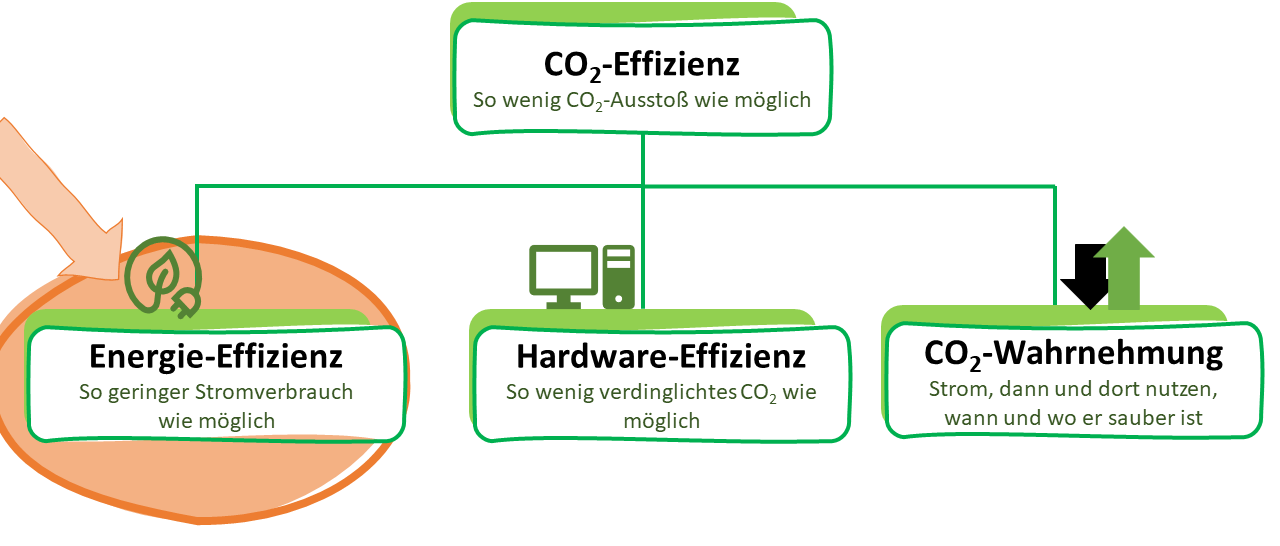
\includegraphics[width=1.00\textwidth]{CO2awa_2.png}				
		\end{overprint}
		\label{fig.co2awa}\infoAbb
\end{frame}


\begin{frame}
\frametitle{\COz-effiziente Software}
\framesubtitle{\href{https://learn.greensoftware.foundation//}{https://learn.greensoftware.foundation/}}
\begin{itemize}
     \item \COz-Effizienz: so wenig \COz~  wie möglich
		 \begin{itemize}
         \item \textbf<2->{Energieeffizienz: möglichst wenig Strom} 
         \item Hardware-Effizienz:  mit möglichst wenig (neuer) Hardware
         \item \COz-Wahrnehmung:  Strom mit der geringsten \COz-Emission
     \end{itemize}
		\pause
    \item Energieproportionalität: Maximierung  der  Energieeffizienz der Hardware
    \item Networking: Reduktion der Datenmenge und der Entfernung im  Netzwerk
    \item Demand Shaping:  \COz-bewusste Anwendungen bevorzugen
    \item \textbf<2->{Messungen: Was man nicht messen kann, kann man auch nicht verbessern.} 
		\item Verpflichtung zum Klimaschutz: Verstehen und umsetzen von Maßnahmen zur \COz-Reduktion
\end{itemize}
\end{frame}

\section{Experiment}
\label{s.exp}

\begin{frame}{Gliederung}
\tableofcontents[currentsection]
\end{frame}

\begin{frame}
\frametitle{Messung}
\framesubtitle{\href{https://learn.greensoftware.foundation/measurement}{https://learn.greensoftware.foundation/measurement}}
\begin{block}{Idee}
What you can't measure, you can't improve.
\end{block}

\pause
\vfill 

Es gibt im groben drei Parameter, die -- unabhängig von der Infrastruktur -- die die \COz-Emissionen beeinflussen:

\begin{itemize}
	\item \textbf<3->{{Wie viel wird Energie verbraucht?}	   }   
				\begin{itemize}
					\item Messungen durch spezifische Werkzeuge, 
					\item wie JoularJX, turbostat etc
\end{itemize}
   \item Wie ist der  Energie-Mix (erneuerbar, fossil)
	\begin{itemize}
		\item der aktuelle oder auch der durchschnittliche
	\end{itemize}
    \item Wie viel Hardware wird benötigt?
\end{itemize}

\end{frame}


\begin{frame}{Laufzeit- und Energieeffizienz}

  Zusammenhang und Unterschiede
	    \begin{itemize}
		    \item Laufzeiteffizienz: Geschwindigkeit und Leistung von Computersystemen\\ Komplexität von Algorithmen\\Qualität der Implementierung
        \item Energieeffizienz: Verbrauchte Energie eines Systems \cite{brown_toward_2010}
        \item \textbf<2->{Keine direkte Proportionalität?? }\\
		           Verbesserte Laufzeiteffizienz bedeutet nicht unbedingt verbesserte Energieeffizienz und umgekehrt?
							
							\begin{itemize}
								\item[Ja]  Direkter Zusammenhang zwischen Energieeffizienz und Performance 
								           \cite{pereira_energy_2017,cascaval_folklore_2014,pinto_energy_2017}\\
													  dann reicht vermutlich die Laufzeitmessung
													
								\item[Nein] Kein direkter Zusammenhang zwischen Energieeffizienz und Performance 
								      \cite{trefethen_energy-aware_2013,lima_haskell_2016} \\
											dann sind neuartige Messungen nötig
							\end{itemize}
		\end{itemize}
									
\end{frame}


\begin{frame}{Ressourcen- und energieeffizienten Software \cite{guldner_development_2024}}
\begin{itemize}
	\item junges Forschungsfeld 
	\item Unsicherheiten und Unklarheiten behindern eigene Messungen
	\item die durch Software verursachten Umweltauswirkungen werden in der Praxis nur selten berücksichtigt 
	\item unterschiedliche Methoden, Werkzeuge, Leitfäden usw. entwickelt
	\item  aber kein umfassender Forschungsrahmen
	\item  keine standardisierten Umsetzung von Messungen in der Industrie
	\item Vorschläge, zB  GSMR in \cite{guldner_development_2024}
\end{itemize}				
\end{frame}


\begin{frame}{Ressourcen- und energieeffizienten Software \cite{GSMR_info_2024}}
\framesubtitle{Green Software Measurement Model (GSMR)}
\begin{columns}
\column{7cm}
\begin{itemize}
	\item   generisches Referenzmodell für ein breites Spektrum von Software 
	\item  das ein Messrahmen, der Methoden, Werkzeuge usw. integriert
	\item für die Kategorisierung, Anpassung und Entwicklung von Methoden für spezifische Messeinstellungen
	\item  integriert die Ergebnisse von 12 Gruppen von Forschern und Praktikern.
\end{itemize}
\column{7cm}
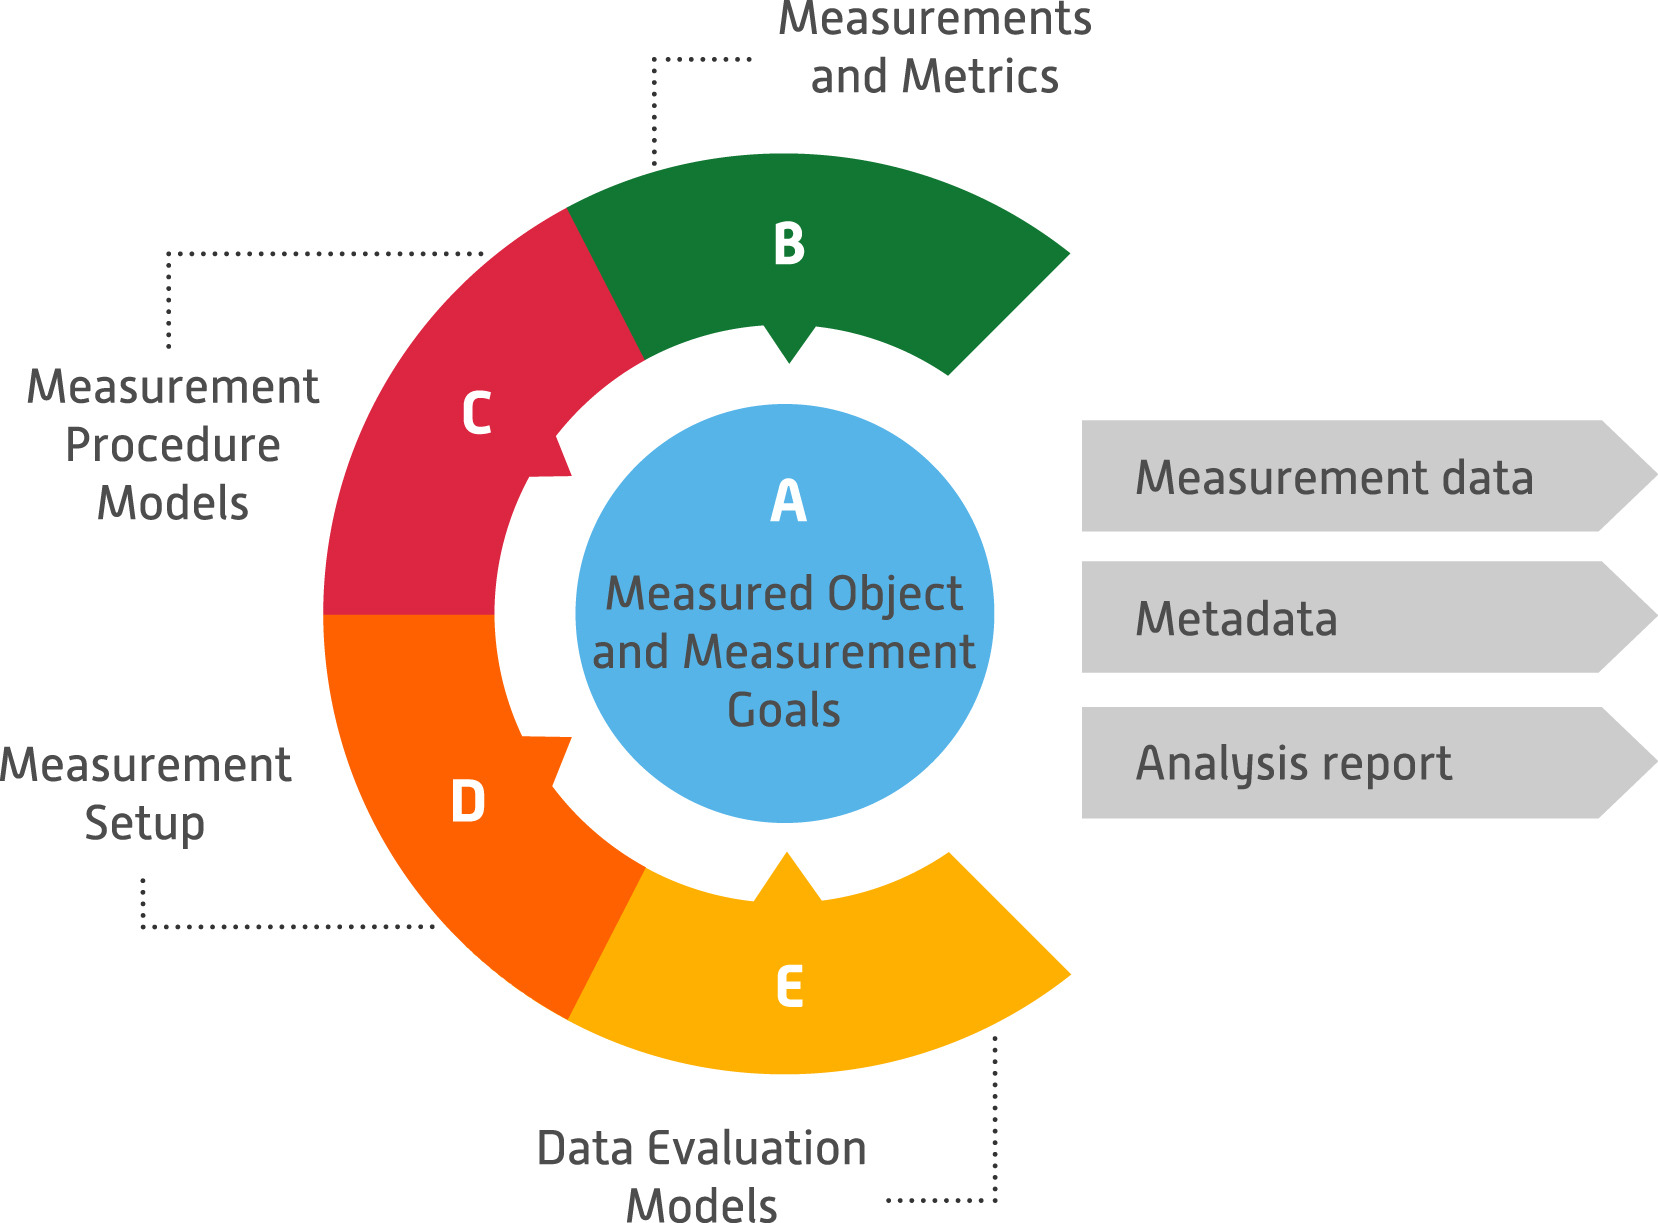
\includegraphics[width=6cm]{GSMM.jpg}\label{fig.GSMM}\\ \hspace*{\fill}\infoAbb
%aus A. Guldner, et al.  Development and evaluation of a reference measurement model for assessing the resource and energy efficiency of software products and components—Green Software Measurement Model (GSMM). In: Future Generation Computer Systems 155 (June 2024) 
%https://www.sciencedirect.com/science/article/pii/S0167739X24000384?via%3Dihub
% CC BY 4.0
%https://s100.copyright.com/AppDispatchServlet?publisherName=ELS&contentID=S0167739X24000384&orderBeanReset=true


\end{columns}
\end{frame}



\begin{frame}{Experiment: Energieeffizienz}
\begin{itemize}
	\item Mögliche Aufgaben\\
	      Feststellung der Energieeffizienz\\
				Vergleich Laufzeit vs. Energieeffizienz
\begin{itemize}
	\item z.B. TSP mit Minimaler-Spannbaum-Heuristik
	\item z.B. \textbf<2->{Eulerkreise}
\end{itemize}
	\item erster Schritt zur ressourceneffizienten Softwareentwicklung 
	\item JUNIT-Tests für die Messung 
	\begin{itemize}
		\item  des Energieverbrauchs
		\item  der Laufzeit
\end{itemize}
	\item Erstellung einer Tabelle  (csv-Datei)  mit
	\begin{itemize}
		\item Spalten unterschiedlich großen Datensätzen
		\item Hardware, IDE,	Java-Version
		\item Korrelationstest (zB in Excel)
			
\end{itemize}
\end{itemize} 
\end{frame}


\begin{frame}{Energiemessung von Software als Experiment}

Vorteile der   Software-Tools 
\begin{itemize}
    \item niedriger Kosten 
    \item geringerer  Aufwand 
		\item detailliertere Informationen auf Prozessebene
    \item  mehr Flexibilität und leichter skalierbar
\end{itemize}
 Mögliche Tools:
\begin{itemize}
	\item JoularJX, PowerJoular
	\item Softwarefootprint.py
	\item turbostat
	\item Hardware-Monitore
	\item Intel Power Gadget \dotfill nicht mehr unterstützt
\end{itemize}
\end{frame}

\begin{frame}{JoularJX}
\framesubtitle{ Energiemessung von und durch Software}
   ~\\\hspace*{\fill}
     \href{https://www.noureddine.org/research/joular/joularjx}%
		      {
\includegraphics[width=0.40\textwidth]{joular.png}}

\begin{itemize}
	\item JoularJX ist ein Software-Energieüberwachungstool
  \item Hilfe für  Softwareentwickler, um den Stromverbrauch 
ihrer Programme zu verstehen und zu analysieren

\end{itemize}
\end{frame}

\begin{frame}{PowerJoular}
\framesubtitle{ Energiemessung von und durch Software}
   ~\\\hspace*{\fill}
	\href{https://www.noureddine.org/research/joular/powerjoular}
	     {
\includegraphics[width=0.60\textwidth]{powerjoular.png}}

\begin{itemize}
	\item Überwachung des Stromverbrauchs des Computers mithilfe RAPL-Schnittstelle.
	\item für Linux (x86 und Raspberry Pis)
	\item Hardwareunterstützung zur Erfassung des Stromverbrauch 
\end{itemize}
in GitHub: \href{https://github.com/joular/powerjoular}{https://github.com/joular/powerjoular}\\
Mehr Infos : \href{https://joular.github.io/powerjoular/}{https://joular.github.io/powerjoular/}

\hspace*{\fill} \cite{noureddine-ie-2022}
\end{frame}

\begin{frame}{Softwarefootprint.py}
\framesubtitle{ Energiemessung von und durch Software}
Skript, dass
\begin{itemize}
	\item   die Prozessstatistiken nach dem Vorkommen  bestimmten Befehle durchsucht,
	\item  deren CPU-Laufzeiten addiert,
	\item  und daraus Energieverbrauch und Treibhausgasemissionen der Software berechnet
	\item für den lokalen Computer.
\end{itemize}

in GitHub \href{https://github.com/oekoj/softwarefootprint}{https://github.com/oekoj/softwarefootprint}
\end{frame}

\begin{frame}{turbostat}
\framesubtitle{ Energiemessung von und durch Software}
  turbostat  \href{https://www.linux.org/docs/man8/turbostat.html}%
	              {\tiny https://www.linux.org/docs/man8/turbostat.html}

	\begin{itemize}
		\item 	erzeugt Berichte über Prozessorfrequenz und Leerlaufstatistiken
	  \item  gibt Auskunft über X86-Prozessoren:
		\begin{itemize}
			\item die Prozessortopologie, 
			\item die Frequenz, 
			\item die Idle-Power-State-Statistik, 
			\item die Temperatur und den Stromverbrauch   
		\end{itemize}
		
	\end{itemize}
\end{frame}

\begin{frame}{Hardware-Monitore}
\framesubtitle{ Energiemessung von und durch Software}
\begin{itemize}
	\item HWMonitor  \href{https://www.cpuid.com/softwares/hwmonitor.html}%
	                      {\tiny https://www.cpuid.com/softwares/hwmonitor.html}
		
		\begin{itemize}
			\item  für Windows auf x86
			\item ermöglicht die Messung des Gesamtstromverbrauchs eines Computers
			\item  ein Hardware-Überwachungsprogramm, für\\
			   Spannungen, Temperaturen, Leistungen, Ströme, Lüftergeschwindigkeiten, Auslastungen, Taktfrequenzen
			\item keine spezifischen Funktionen zur Überwachung einzelner Prozesse oder Programme.
		\end{itemize}
												

\item Open Hardware Monitor  \href{https://openhardwaremonitor.org/}{\tiny https://openhardwaremonitor.org/}
\begin{itemize}
	\item funktioniert auf Windows und auf Linux mit Einschränkungen\\ \hspace*{\fill}
	        da es dort teilweise weniger Sensorinformationen bereitstellt
					
   \item  ähnlich dem HWMonitor
	\item  ermöglicht primär die Messung des Gesamtstromverbrauchs eines Computers
			\item keine spezifischen Funktionen zur Überwachung einzelner Prozesse oder Programme
\end{itemize}
\end{itemize}
\end{frame}

\section{Ausblick}
\label{s.ausblick}

\begin{frame}{Gliederung}
\tableofcontents[currentsection]
\end{frame}

\begin{frame}{Fazit}
\begin{itemize}
	\item  Energieverbrauch durch IT ist erheblich
	\item (\COz-) effiziente Software nötig 
	\item Neues Forschungsgebiet: Messungen der Energieeffizienz von Software
	\item Eigene Messungen als Experiment möglich
\end{itemize}
\end{frame}


\begin{frame}{Ausblick: Energieproportionalität \cite{wong_retrospective_2015}}
				\begin{itemize}
					\item Verhältnis von Leistungsverbrauch zur nützlichen Arbeit
					\item  Energieproportionalität als Brücke zwischen Zeit- und Energieeffizienz
				\item Einsatz Energieproportionalität
				 \begin{itemize}
					 \item Verbesserte Energieeffizienz 
					 \item Reduzierte Kosten 
					 \item \textbf<2->{nicht für als Maßeinheit für Implementierungen }\\sondern nur für gesamte Systeme sinnvoll
					\end{itemize}
			\end{itemize}
\end{frame}
